\documentclass{article}




\usepackage{fullpage}
%\usepackage{nopageno}
\usepackage{amsmath}
\usepackage{amsfonts}
\usepackage{graphicx}
\usepackage{framed}
\usepackage{algorithmic}
\usepackage{xcolor}

\definecolor{dark_red}{rgb}{0.5,0.0,0.0}
\definecolor{dark_green}{rgb}{0.0,0.5,0.0}
\definecolor{dark_blue}{rgb}{0.0,0.0,0.5}
\definecolor{blue}{rgb}{0.0,0.0,1.0}

\newcommand{\dr}[1]{\textcolor{dark_red}{#1}}
\newcommand{\dg}[1]{\textcolor{dark_green}{#1}}
\newcommand{\db}[1]{\textcolor{dark_blue}{#1}}
\newcommand{\blue}[1]{\textcolor{blue}{#1}}


\title{MATH2860 - 01 Project \#2}
\date{Summer 2021}

\begin{document}

\maketitle

\begin{center}
\begin{tabular}{cc}
\parbox{0.5\textwidth}{
This project will involve the analysis of elastic meshes, also referred to as lattices. Given a system of elastic beams connected by rigid joints, the deformation of such structures under known forces will be analyzed. 
} & \parbox{0.5\textwidth}{
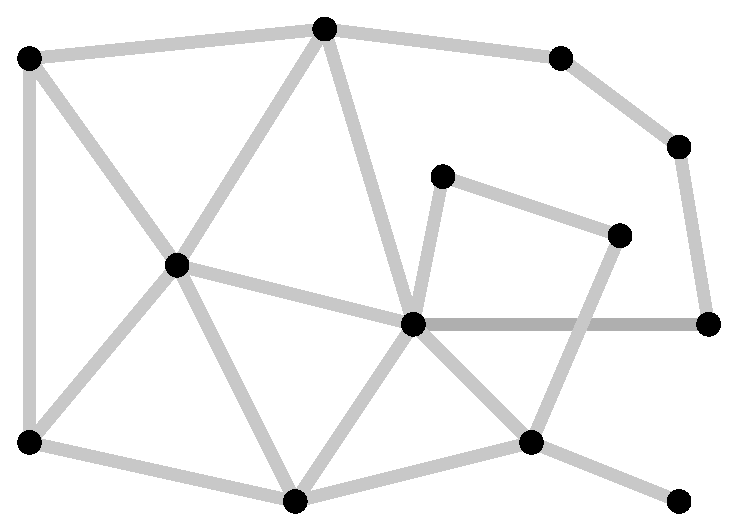
\includegraphics[width = 0.5\textwidth]{elastic_mesh_example}
}
\end{tabular}
\end{center}



\section{Terminology}

The mathematical model used in this project will use the following terminology:

\begin{description}
\item[node] A ``node" is a junction between 1 or more elastic beams. There are two types of nodes: anchored nodes and free floating nodes.
\item[anchored node] An ``anchored node", also referred to as a ``grounded node" borrowing terminology from electrical circuits, is node whose position and torsion is fixed.
\item[floating node] A ``floating node" is a node whose position can change as the connecting beams deform under stress. 
\item[bream] A ``beam" is an elastic rod that connects two floating nodes, or a floating node with an anchored node. If one the nodes is anchored, then the beam is referred to as an ``anchored beam". In this mathematical model, the beams will be subject to tension, compression, shear, twisting, and bending. Beams will also be rotationally symmetric.
\item[stress] ``Stress" is a measure of the forces acting on a structure that cause it to deform. There are two types of stress: force and torque.
\begin{description}
\item[force] ``Force" is a straightforwards force that attempts to move a node in a straight line direction. Force is quantified by a simple 3D vector.
\item[torque] ``Torque" is a twisting force that attempts to rotate a node. When torque is quantified as a 3D vector, its direction is the axis around which the twist is being applied, and it magnitude is the strength of the twist.  
\end{description}   
\item[strain] ``Strain" is a measure of the deformation a structure undergoes when subjected to stress. There are two categories of strain: displacement and torsion.
\begin{description}
\item[displacement] ``Displacement" is a measure of the new position of a node relative to its original position. Displacement is quantified by a simple 3D vector.   
\item[torsion] ``Torsion" is a measure of the nodes rotation in response to the stress. When torsion is quantified as a 3D vector, its direction is the axis around which the rotation is being applied, and it magnitude is the amount of rotation.  
\end{description}
\end{description}

{\bf The large scale relationship between stress and strain is not linear. If the strains are small however, a linear approximation can be used to great effect, and this is the approach that will be used in this project.}



\section{Torsion}

Rotations such as torsion and torque are quantified by 3D vectors. The direction of the vector is the axis of the rotation/twist. The magnitude of the vector is the amount of counterclockwise rotation/twist, which is measured in radians. The direction of counterclockwise is determined by viewing the axis vector in the opposite direction. If the twist is clockwise, the direction of the axis is simply flipped. 

Torsion can be decomposed into \(x\), \(y\), and \(z\) components. Consider the small torsion vector \(\Delta\omega = \begin{bmatrix} \Delta\omega_x \\ \Delta\omega_y \\ \Delta\omega_z \end{bmatrix}\). {\bf It will be assumed that \(\Delta\omega\) is small,} which it is to say that the magnitude of \(\Delta\omega\) is considerably less than \(1\). 

The component \(\Delta\omega_x\) measures counterclockwise twist around the \(x\) axis, as depicted by the red circle below. This moves the elementary basis vectors by the following amounts:
\begin{itemize}
\item \(\begin{bmatrix} 1 \\ 0 \\ 0 \end{bmatrix}\) does not move from the \(x\)-axis twist.
\item \(\begin{bmatrix} 0 \\ 1 \\ 0 \end{bmatrix}\) moves to \(\begin{bmatrix} 0 \\ 1 \\ 0 \end{bmatrix} + \begin{bmatrix} 0 \\ 0 \\ \Delta\omega_x \end{bmatrix}\) from the \(x\)-axis twist.
\item \(\begin{bmatrix} 0 \\ 0 \\ 1 \end{bmatrix}\) moves to \(\begin{bmatrix} 0 \\ 0 \\ 1 \end{bmatrix} + \begin{bmatrix} 0 \\ -\Delta\omega_x \\ 0 \end{bmatrix}\) from the \(x\)-axis twist.
\end{itemize}   
The component \(\Delta\omega_y\) measures counterclockwise twist around the \(y\) axis, as depicted by the green circle below. This moves the elementary basis vectors by the following amounts:
\begin{itemize}
\item \(\begin{bmatrix} 1 \\ 0 \\ 0 \end{bmatrix}\) moves to \(\begin{bmatrix} 1 \\ 0 \\ 0 \end{bmatrix} + \begin{bmatrix} 0 \\ 0 \\ -\Delta\omega_y \end{bmatrix}\) from the \(y\)-axis twist.
\item \(\begin{bmatrix} 0 \\ 1 \\ 0 \end{bmatrix}\) does not move from the \(y\)-axis twist.
\item \(\begin{bmatrix} 0 \\ 0 \\ 1 \end{bmatrix}\) moves to \(\begin{bmatrix} 0 \\ 0 \\ 1 \end{bmatrix} + \begin{bmatrix} \Delta\omega_y \\ 0 \\ 0 \end{bmatrix}\) from the \(y\)-axis twist.
\end{itemize}   
The component \(\Delta\omega_z\) measures counterclockwise twist around the \(z\) axis, as depicted by the blue circle below. This moves the elementary basis vectors by the following amounts:
\begin{itemize}
\item \(\begin{bmatrix} 1 \\ 0 \\ 0 \end{bmatrix}\) moves to \(\begin{bmatrix} 1 \\ 0 \\ 0 \end{bmatrix} + \begin{bmatrix} 0 \\ \Delta\omega_z \\ 0 \end{bmatrix}\) from the \(z\)-axis twist.
\item \(\begin{bmatrix} 0 \\ 1 \\ 0 \end{bmatrix}\) moves to \(\begin{bmatrix} 0 \\ 1 \\ 0 \end{bmatrix} + \begin{bmatrix} -\Delta\omega_z \\ 0 \\ 0 \end{bmatrix}\) from the \(z\)-axis twist.
\item \(\begin{bmatrix} 0 \\ 0 \\ 1 \end{bmatrix}\) does not move from the \(z\)-axis twist.
\end{itemize}   

\begin{center}
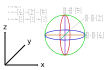
\includegraphics[width = \textwidth]{infinitesimal_torsion}
\end{center}

Given an arbitrary vector \(\mathbf{v} = \begin{bmatrix} v_x \\ v_y \\ v_z \end{bmatrix} = v_x\begin{bmatrix} 1 \\ 0 \\ 0 \end{bmatrix} + v_y\begin{bmatrix} 0 \\ 1 \\ 0 \end{bmatrix} + v_z\begin{bmatrix} 0 \\ 0 \\ 1 \end{bmatrix}\), the new position of \(\mathbf{v}\) is 
\[\mathbf{v} + \begin{bmatrix} \Delta\omega_y \cdot v_z - \Delta\omega_z \cdot v_y \\ \Delta\omega_z \cdot v_x - \Delta\omega_x \cdot v_z \\ \Delta\omega_x \cdot v_y - \Delta\omega_y \cdot v_x \end{bmatrix} 
= \mathbf{v} + \begin{bmatrix} 0 & -\Delta\omega_z & \Delta\omega_y \\ \Delta\omega_z & 0 & -\Delta\omega_x \\ -\Delta\omega_y & \Delta\omega_x & 0 \end{bmatrix}\begin{bmatrix} v_x \\ v_y \\ v_z \end{bmatrix} 
= \mathbf{v} + \begin{bmatrix} 0 & v_z & -v_y \\ -v_z & 0 & v_x \\ v_y & -v_x & 0 \end{bmatrix}\begin{bmatrix} \Delta\omega_x \\ \Delta\omega_y \\ \Delta\omega_z \end{bmatrix}\]
What is important to note is that the change in the vector \(\mathbf{v}\) is a {\bf linear} function of \(\Delta\omega\), provided that \(\Delta\omega\) is small. 



\section{The linear model}

The strain on each node will be quantified by a small displacement \(\Delta\mathbf{q}\), and a small torsion \(\Delta\omega\). The displacement \(\Delta\mathbf{q}\) is the node's position relative to its original position in the undeformed mesh. The torsion \(\Delta\omega\) is the node's rotation relative to its original rotation. Given \(N\) floating nodes, the total strain can be quantified by the following \(6N\) component vector. Each node corresponds to \(6\) components (the superscript \(T\) means transpose, and is invoked to simplify the notation):

\[\textbf{strain} = \begin{bmatrix} \Delta\mathbf{q}_1^T & \Delta\omega_1^T & \Delta\mathbf{q}_2^T & \Delta\omega_2^T & \cdots & \Delta\mathbf{q}_N^T & \Delta\omega_N^T \end{bmatrix}^T\] 

The stress on each node will be quantified by a force \(\mathbf{F}\), and a torque \(\tau\). The total stress can be quantified by the following \(6N\) component vector. Each node corresponds to \(6\) components:

\[\textbf{stress} = \begin{bmatrix} \mathbf{F}_1^T & \tau_1^T & \mathbf{F}_2^T & \tau_2^T & \cdots & \mathbf{F}_N^T & \tau_N^T \end{bmatrix}^T\] 

While not discussed here, the stress and strain are related by a \(6N \times 6N\) stiffness matrix \(A\):

\[\textbf{stress} = A \cdot \textbf{strain}\]

The stress is known, the strain is what is to be computed, so the linear system is to be solved to give:

\[\textbf{strain} = A^{-1}\textbf{stress}\]

Again, the linear model is only accurate for small strains.



\section{The 4 types of strain}


When assessing the strain on each individual beam, there are 4 types of strain on each beam that will be addressed by this model. Displacement strain refers to the change in the displacement between the two end points of the beam, adjusting for rotation. Torsion strain refers to the change in torsion between the two end points of the beam. Strain can also be discriminated between whether it is parallel or perpendicular to the beam, which gives a total of 4 categories of strain: 
\begin{itemize}
\item \textbf{tension/compression strain}, also referred to as parallel strain, refers to stretching or squeezing the beam in a direction that is parallel to the original direction, as depicted below. 
\item \textbf{shear strain} refers to distorting the beam in a direction that is perpendicular to its original direction, as depicted below.
\item \textbf{twisting} refers to twisting the beam along an axis that is parallel to the beam.
\item \textbf{bending} refers to bending the beam along an axis that is perpendicular to the beam.  
\end{itemize}
A beam may be subject to all \(4\) types of strain at once.

\begin{center}
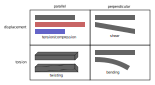
\includegraphics[width = 0.75\textwidth]{_4_types_of_strain}
\end{center}


%\section{The Matlab model}







\section{The assignment}

The goal of this project is to design an elastic mesh/lattice that will achieve a specific goal.

You are provided with the Matlab .m file ``\texttt{project\_2\_MATLAB\_bridge\_builder.m}" which implements a linear model relating the strains and stresses described above. No changes are to be made to this file, however you may wish to change the input file name on line 36 to any input file of your choosing if you wish to experiment with multiple designs. You are also provided with the Matlab .m file ``\texttt{design\_basic.m}" which is the input file that you will modify as you implement your design. 

The task will be to design a lattice with the following properties. 
\begin{itemize}
\item You are provided with \(4\) anchored nodes at the coordinates \((0, -0.5, -0.5)\), \((0, +0.5, -0.5)\), \((0, -0.5, +0.5)\), and \((0, +0.5, +0.5)\). These nodes have the respective names ``\texttt{anchor 1}", ``\texttt{anchor 2}", ``\texttt{anchor 3}", and ``\texttt{anchor 4}". {\bf No additional anchored nodes may be defined.}
\item You are provided with a floating node at the coordinates \((8.0, 0.0, 0.0)\), with the name ``\texttt{loaded point}". This node is subjected to a downwards force of \(\begin{bmatrix} 0.0 \\ 0.0 \\ -0.1 \end{bmatrix}\), and no torque. {\bf This node and force is what your lattice must support.}
\item You are to add additional nodes. None of the introduced nodes may have external forces or torques applied. 
\item You are to insert beams between the defined floating nodes necessary to support the loaded point. 
\item No beam may be more than \(3\) units in length. 
\item The beams have weight and will be subject to gravity. The weight of each beam is proportional to its length and thickness. Your design must account for this. 
\item Your design must have no failures (to be described later).
\end{itemize}



\subsection{Input syntax}

Below is listed the input variables that the user will supply for the provided Matlab script.

\begin{itemize}
\item ``\texttt{g\_nodes}" is an array of anchored nodes. Each anchored node has the following properties:
	\begin{itemize}
	\item ``\texttt{name}" is a string denoting the node's name. No two nodes may have the same name. The name is used to refer to the node when defining the beams.
	\item ``\texttt{x}" is the node's \(x\)-coordinate.
	\item ``\texttt{y}" is the node's \(y\)-coordinate.
	\item ``\texttt{z}" is the node's \(z\)-coordinate.
	\end{itemize}
\item ``\texttt{nodes}" is an array of floating nodes. Each floating node has the following properties:
	\begin{itemize}
	\item ``\texttt{name}" is a string denoting the node's name. No two nodes may have the same name, nor can there be any overlap with the names of the anchored nodes. The name is used to refer to the node when defining the beams.
	\item ``\texttt{x}" is the node's \(x\)-coordinate.
	\item ``\texttt{y}" is the node's \(y\)-coordinate.
	\item ``\texttt{z}" is the node's \(z\)-coordinate.
	\item ``\texttt{F\_x}" is the \(x\) component of the external force that is acting on the node.
	\item ``\texttt{F\_y}" is the \(y\) component of the external force that is acting on the node.
	\item ``\texttt{F\_z}" is the \(z\) component of the external force that is acting on the node.
	\item ``\texttt{tau\_x}" is the \(x\) component of the external torque that is acting on the node.
	\item ``\texttt{tau\_y}" is the \(y\) component of the external torque that is acting on the node.
	\item ``\texttt{tau\_z}" is the \(z\) component of the external torque that is acting on the node.
	\end{itemize}
\item ``\texttt{beams}" is an array of beams. Each beam has the following properties:
	\begin{itemize}
	\item ``\texttt{start}" is the name of one of the beam's end nodes.
	\item ``\texttt{end}" is the name of the beam's other end node.
	\item ``\texttt{t}" is the beam's thickness. Doubling the thickness of a beam is functionally equivalent to creating two copies of the same beam.
	\end{itemize}
\end{itemize}
To create an anchored node in the input file, the following Matlab syntax is used:
\[\texttt{struct('name', \(???\), 'x', \(???\), 'y', \(???\), 'z', \(???\))}\]
To create a floating node in the input file, the following Matlab syntax is used:
\begin{align*}
& \texttt{struct('name', \(???\), 'x', \(???\), 'y', \(???\), 'z', \(???\), 'F\_x', \(???\), 'F\_y', \(???\), 'F\_z', \(???\),} \\ 
& \quad\quad\quad \texttt{ 'tau\_x', \(???\), 'tau\_y', \(???\), 'tau\_z', \(???\))}
\end{align*}
To create a beam in the input file, the following Matlab syntax is used:
\[\texttt{struct('start', \(???\), 'end', \(???\), 't', \(???\))}\]



\subsection{Output details}

Upon running the Matlab script ``\texttt{project\_2\_MATLAB\_bridge\_builder.m}", \(5\) 3D plots will be displayed. 

\begin{itemize}
\item In all plots, the black circles mark the anchored nodes, and gray circles mark the floating nodes.
\item The plot labeled ``Undeformed lattice" illustrates the lattice without any changes due to the forces acting upon it. The fine green lines emanating from each node indicate the direction of the total external forces acting on the node. The magnitude of each total external force is not part of the display however.    
\item The other \(4\) plots display the lattice in a deformed state. The yellow fine lines depict the torsion on each node. The direction of the yellow line is the axis of rotation, while the length is the amount of counterclockwise rotation. The strain on each beam is indicated by the beam's color. Undeformed beams are black, and gradually change red as they approach their breaking point. {\bf When a beam turns orange, it has failed (snapped) and the current deign is not considered feasible.} Each plot maps a different type of strain, namely parallel strain (tension/compression); shear strain; twist strain; and bending strain, and no failures should be observed on any of the plots. 
\item In the case of the parallel strain plot, tension turns the beam red, while compression turns the beam blue. {\bf A teal beam is a beam that has been crushed by compression and has consequentially failed.}   
\end{itemize}

In summary, no orange or teal beams should be observed in any of your plots to have a feasible design. 

The following image shows an example design that is failing thanks to bending strain. Note the orange beams.
\begin{center}
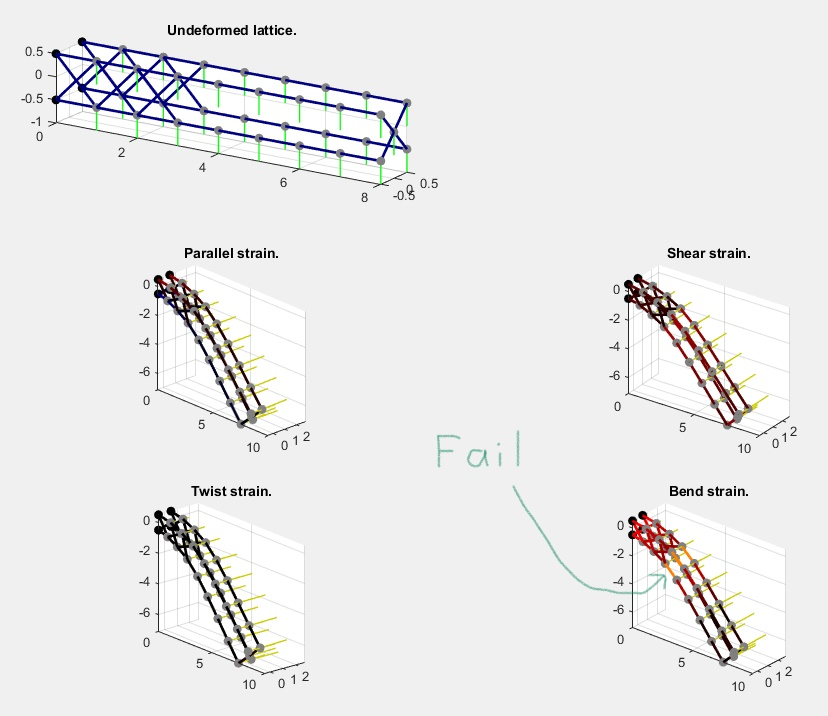
\includegraphics[width =\textwidth]{Example_output_annotated.jpg}
\end{center}

{\bf It should be noted that the strain is being computed using a linear model.} This model is accurate for small strains, but as strains become large, the model becomes unrealistic. 



\subsection{Tips and tricks}

\begin{itemize}
\item For every defined floating node, there must exist a path to an anchored node by traversing some sequence of beams. If this is not the case, the linear system will not have a unique solution, if any solution at all, and the simulation will fail.    
\item The beams are superior at resisting tension/compression stresses, but weak against shear stresses, twisting stresses, and bending stresses. To take advantage of the beams' natural strength, the use of a triangular lattice is recommended.   
\item If a beam is breaking, try increasing the thickness or introduce more diagonal trusses to relieve shear and bending strain.
\item If a beam is not experiencing much strain, its thickness may be reduced to save on weight.
\item A beam's strength is proportional to its thickness, however the beam's weight is also proportional to its thickness so thickening beams at the tip of your truss may not be as advantageous as thickening beams closer to the anchored nodes. 
\item When thickening a beam, the increase in strength and the increase in weight will normally cancel out each others effects. However, with greater beam weight, the load at the ``\texttt{loaded point}" becomes less significant and can be increasingly ignored.  
\end{itemize}






\end{document}












